\documentclass[a4paper]{article}
\usepackage{graphicx}
\usepackage{amsmath}
\usepackage{amsmath}
\usepackage[section]{placeins}
\usepackage{geometry}
 \geometry{
 a4paper,
 total={150mm,257mm},
 top=20mm,
 }
\begin{document}

\begin{figure}
	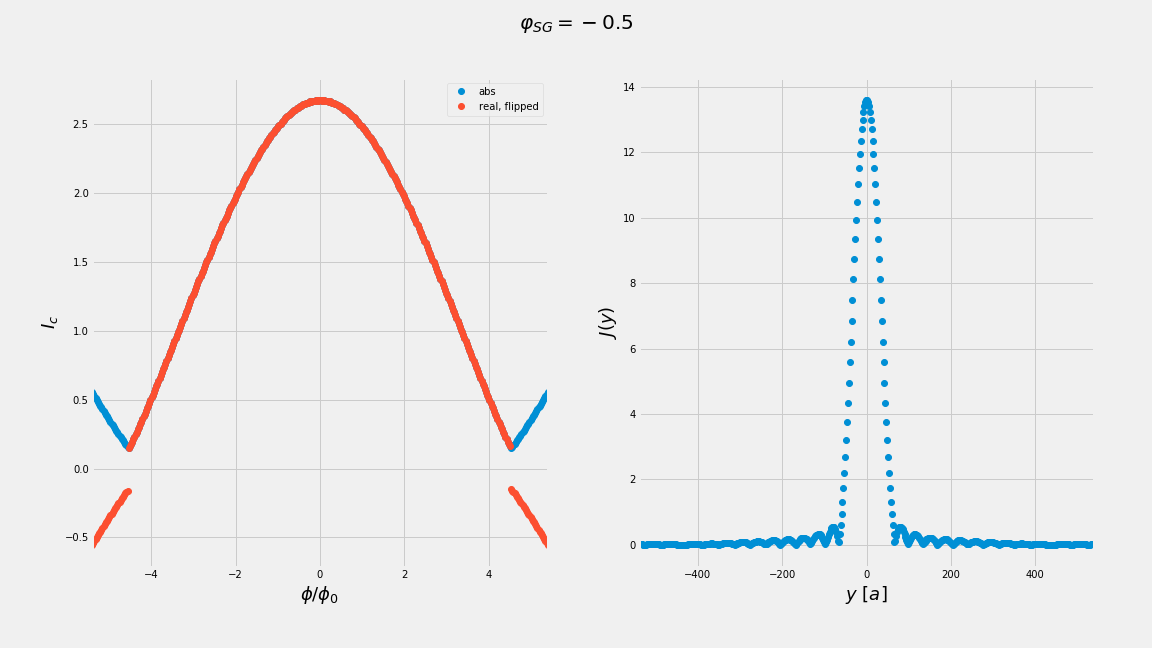
\includegraphics[width=0.9\textwidth]{figs/wg32vbg05/current_and_density_05}
	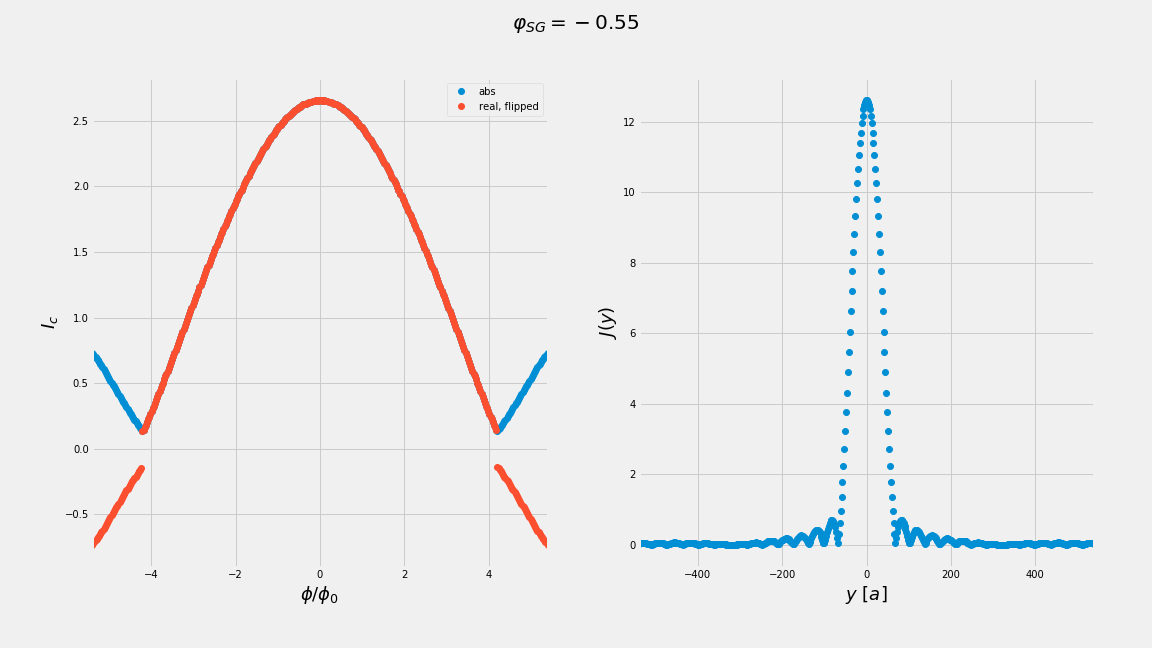
\includegraphics[width=0.9\textwidth]{figs/wg32vbg05/current_and_density_055}
	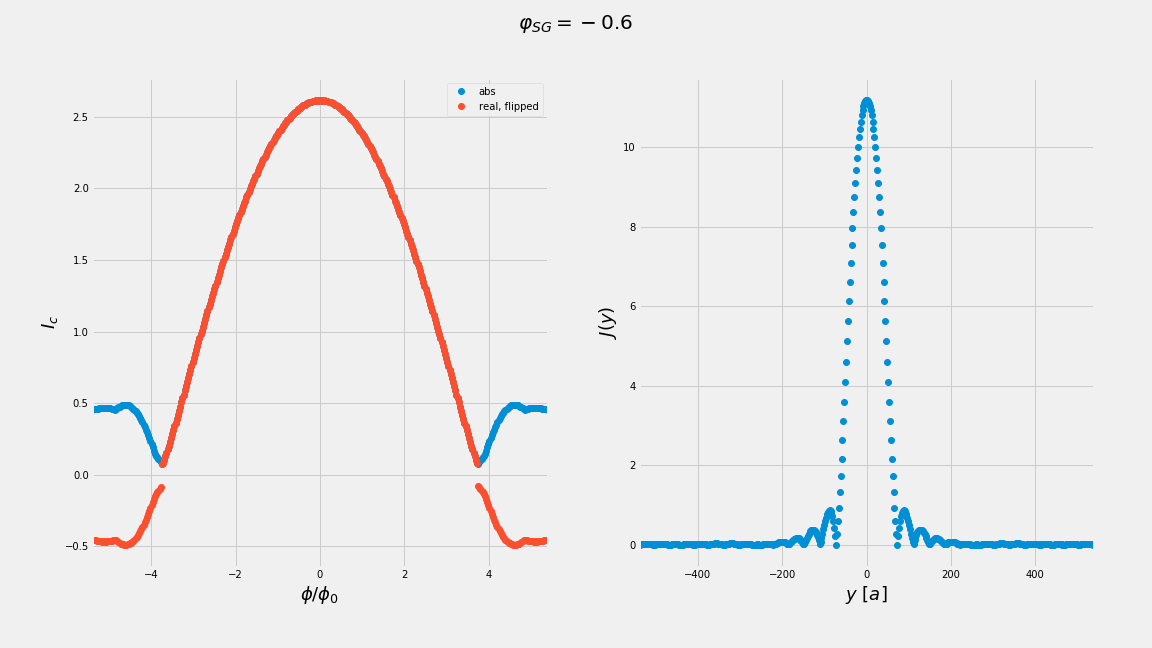
\includegraphics[width=0.9\textwidth]{figs/wg32vbg05/current_and_density_06}
\end{figure}
\begin{figure}
	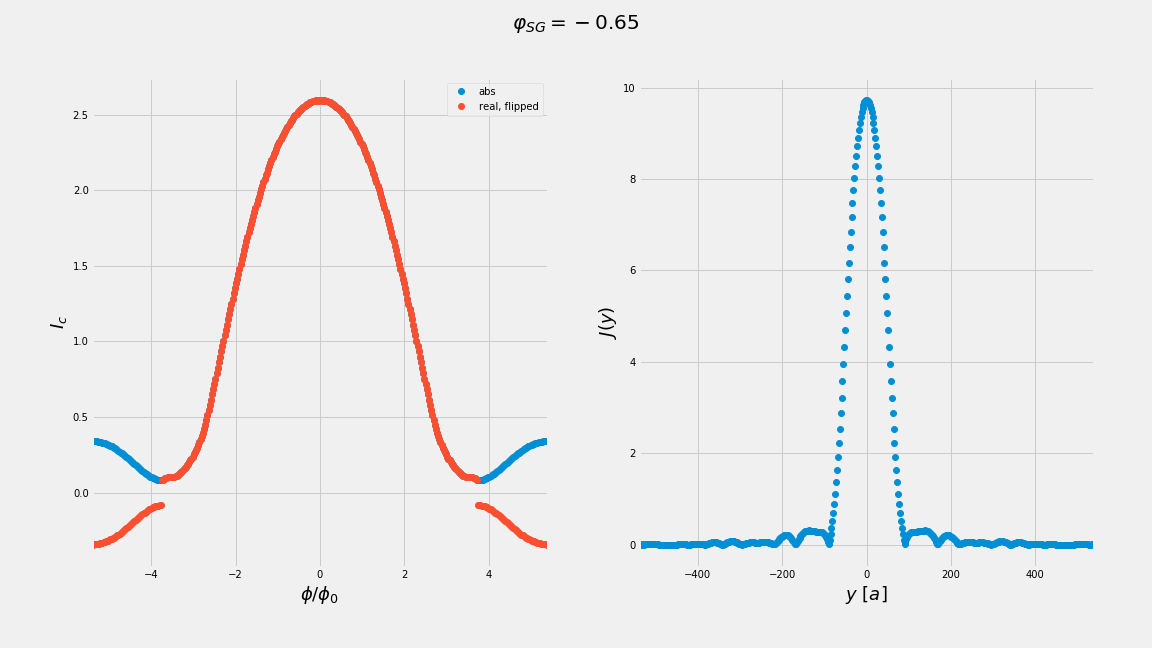
\includegraphics[width=0.9\textwidth]{figs/wg32vbg05/current_and_density_065}
	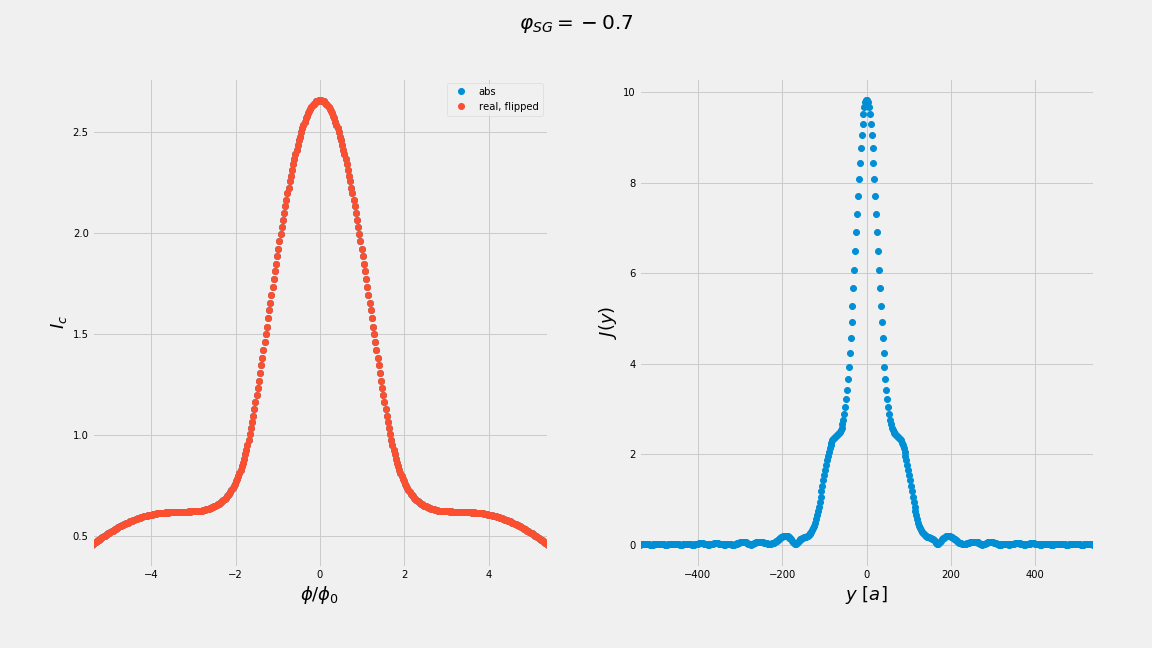
\includegraphics[width=0.9\textwidth]{figs/wg32vbg05/current_and_density_07}
	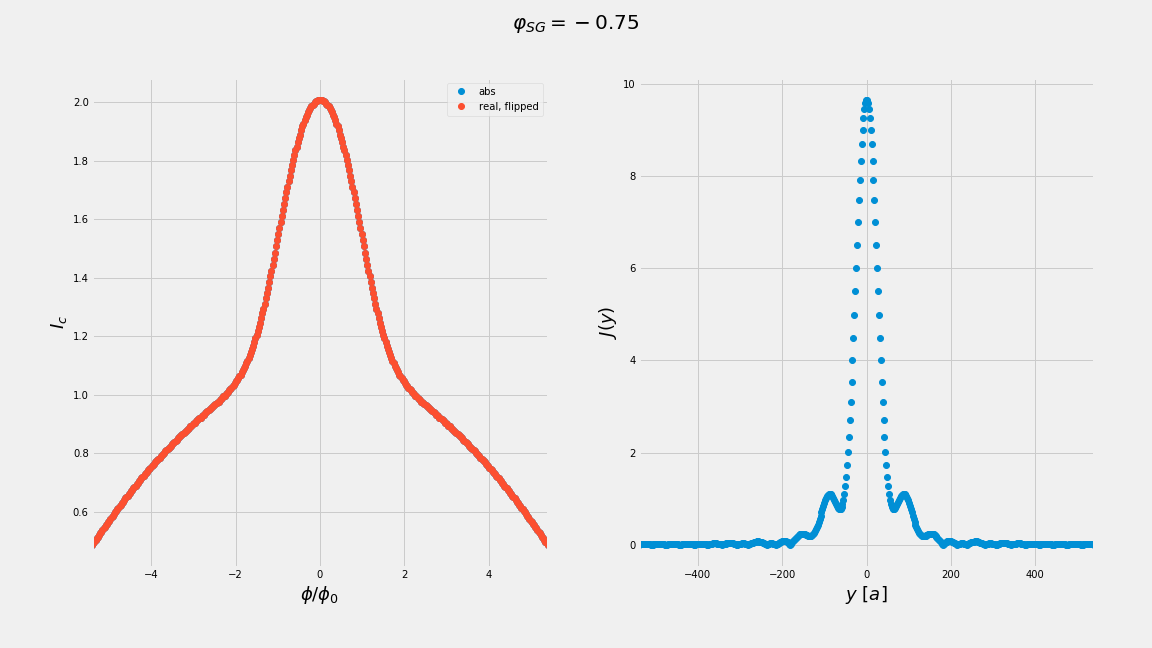
\includegraphics[width=0.9\textwidth]{figs/wg32vbg05/current_and_density_075}
\end{figure}
\begin{figure}
	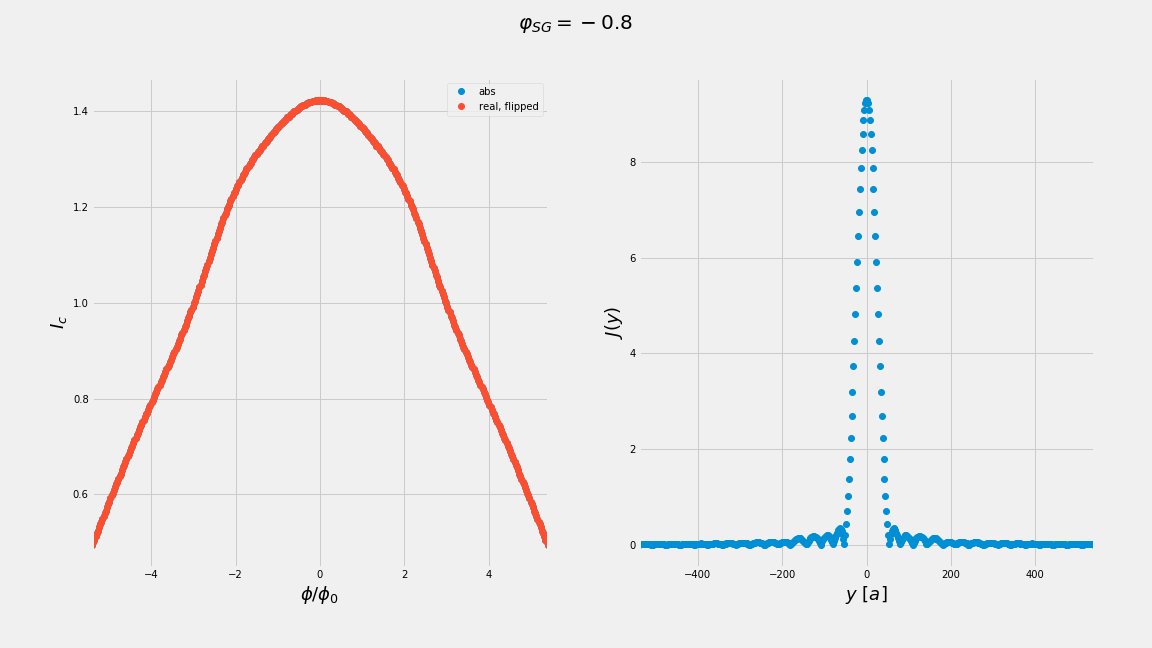
\includegraphics[width=0.9\textwidth]{figs/wg32vbg05/current_and_density_08}
	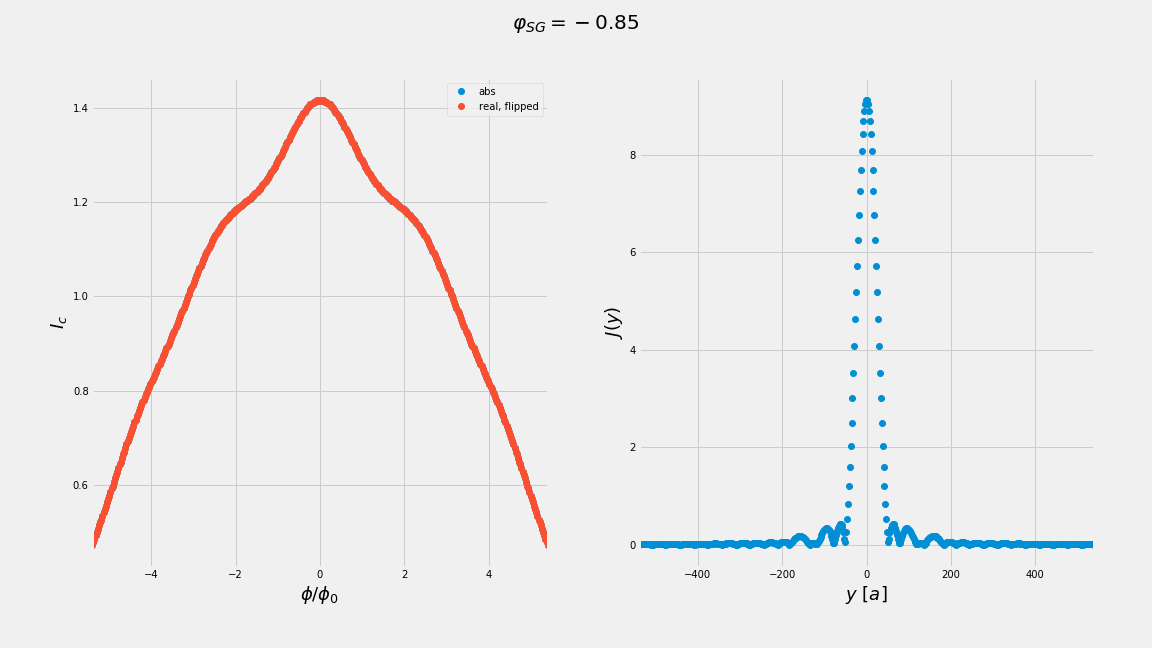
\includegraphics[width=0.9\textwidth]{figs/wg32vbg05/current_and_density_085}
	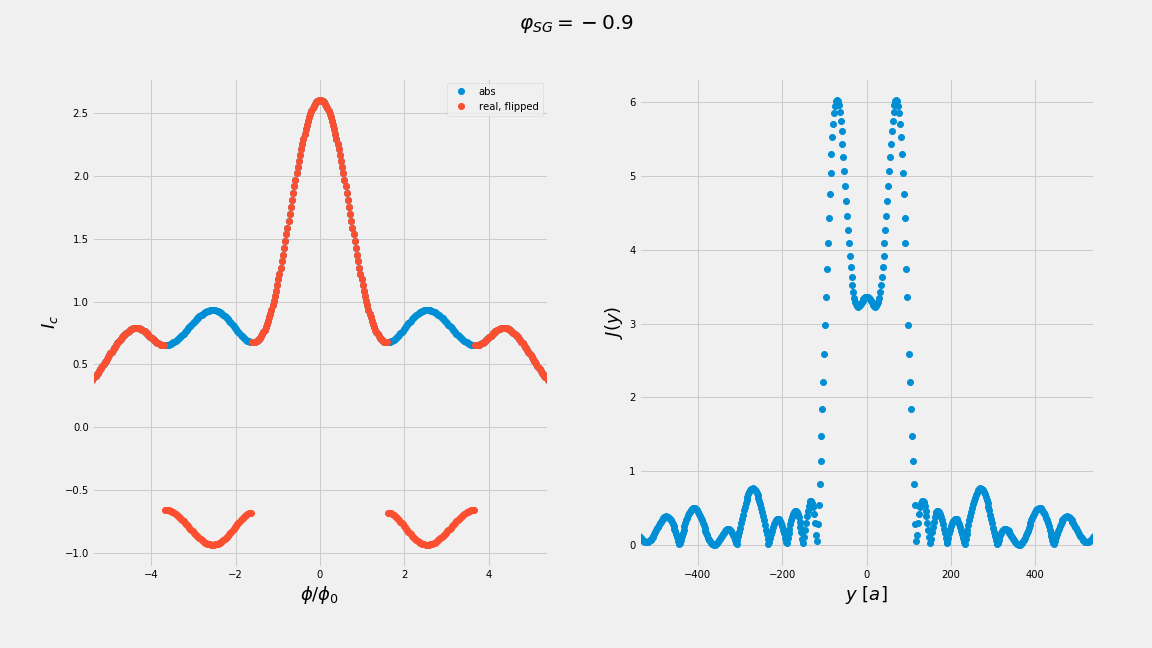
\includegraphics[width=0.9\textwidth]{figs/wg32vbg05/current_and_density_09}
\end{figure}
\begin{figure}
	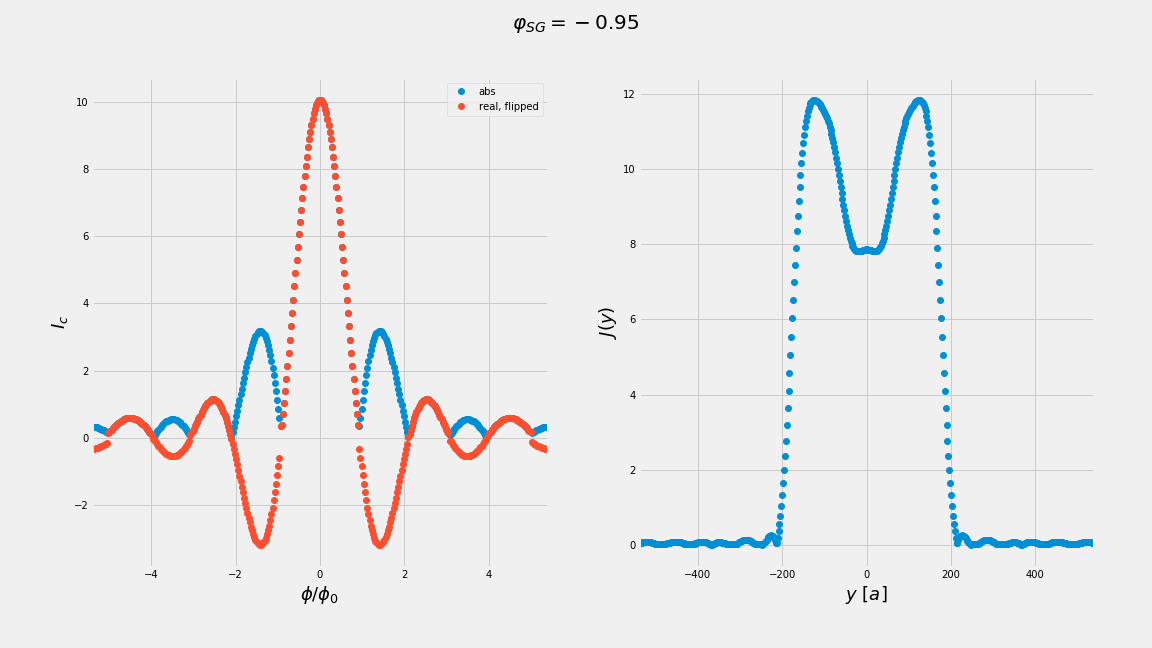
\includegraphics[width=0.9\textwidth]{figs/wg32vbg05/current_and_density_095}
\end{figure}
\end{document}
